
% \begin{figure}
%     \centering
%     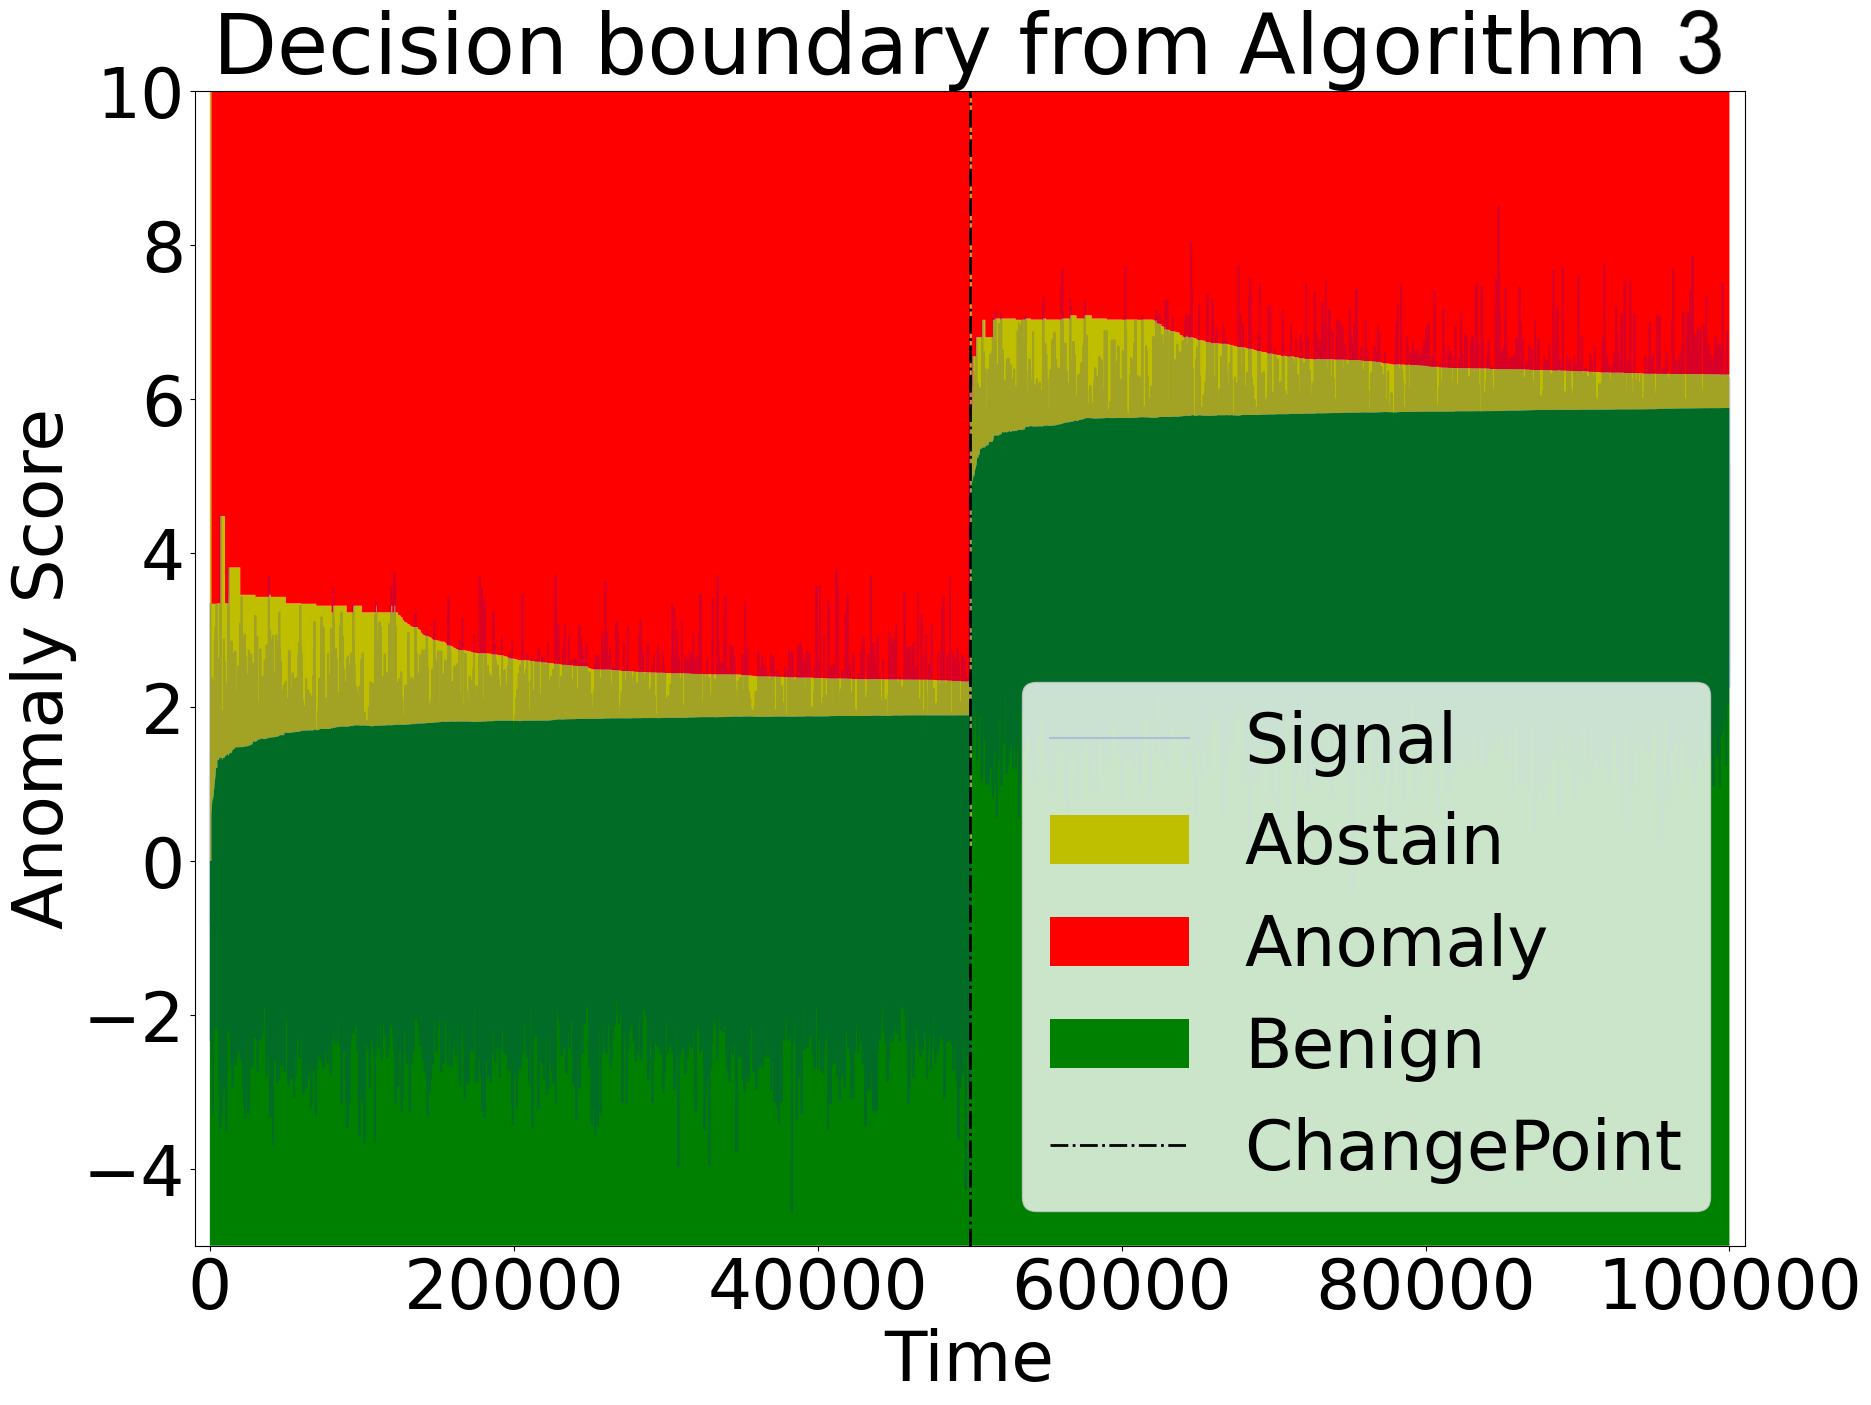
\includegraphics[width=0.55\linewidth]{anomaly/figs/algo_2_example.png}
%     \caption{Algorithm 3 output on a piece-wise stationary stream. \sofi{remake this figure}}
%     \label{fig:s1}
%     \vspace{-1.5em}
% \end{figure}

Going beyond the  i.i.d. case, we consider a piece-wise stationary stream without offline dataset.
Our method in Algorithm \ref{alg:two} uses a change-point detection Algorithm \ref{alg:change_point} from \cite{shekhar2023sequential} as a sub-routine. We need a  definition to state the main result of this section. %Algorithm \ref{alg:change_point} is the forward-backward CS strategy from \cite{shekhar2023sequential}, where a change-point is detected at time $t$, if there exists $1 \leq \tau < t$ with $C(p,\alpha,S_{1:\tau})$ and $C(p,\alpha,S_{\tau+1:t-1})$ having an empty intersection.
% We set additional notation to describe the algorithm. Given the data-stream $(S_t)_{t \geq 1}$ and $t_1 < t_2$ integers, define the set $C(p,\alpha,S_{t_1:t_2})\subseteq \mathbb{R}$ as 
%     \begin{multline}
%         C(p, \alpha, S_{t_1:t_2}) = \bigg[ \widehat{Q}(p-u_{t_2-t_1+1}(\alpha); S_{t_1:t_2}), \\  \widehat{Q}(p+u_{t_2-t_1+1}(\alpha); S_{t_1:t_2}) \bigg].
%         \label{eqn:modified_cs}
%    \end{multline}
% The definition in Equation (\ref{eqn:modified_cs}) is a generalization of the definition in Equation (\ref{eq:cs}) that changes the starting index from $1$ to $t_1$.
%Algorithm \ref{alg:two} detects a change at time $t$, if there exists $1 \leq \tau < t$ such that $C(p,\alpha,S_{1:\tau})$ and $C(p,\alpha,S_{\tau+1:t})$ are non-intersecting, 
%When a change is detected, Algorithm \ref{alg:two} restarts the stationary algorithm. %The full pseudo-code is given in Algorithm \ref{alg:two}. 
%process, a common framework as seen in \cite{sankararaman2023online}.

% \begin{definition}(Piece-wise stationary process) Let $T$ be the time horizon and let $H_T < T$ be the total number of change points. Define a set of strictly increasing time indices  $1 < \tau_1 < \tau_2 \cdots < \tau_{H_T}$ as change points; let $\tau_0 = 0$ and $ \tau_{H_T+1} = T$. The process, $S_1, \cdots, S_T$ is  identified by the quadruple $\Bigl(T,H_T, (\tau_c)_{c=0}^{H_T}, (f_c)_{c=0}^{H_T}\Bigr)$, such that $\forall k \in [1, H_T]$:
% \begin{itemize}[noitemsep,topsep=-3pt,labelwidth=!, labelindent=0pt]
%    \item $\forall t \in [\tau_k,\tau_{k+1})$, $S_t \sim f_k$ i.i.d., with the $p$-quantile of distribution $f_k$ denoted as $ Q_k$
%     \item  $Q_k \neq Q_{k+1}$
% \end{itemize}
% \label{def:piecewise}
% \end{definition}

% \begin{figure}[h!]
%     \centering
%     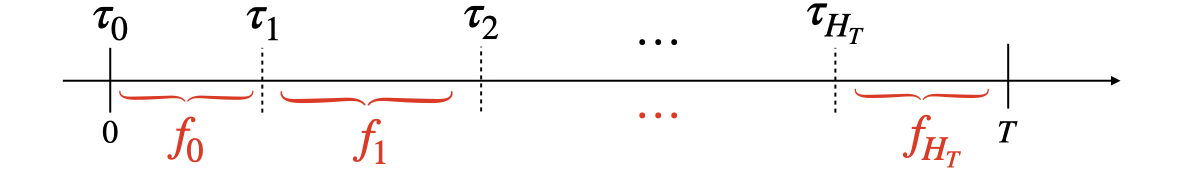
\includegraphics[width=0.9\linewidth]{anomaly/figs/piecewise.jpeg}
%     \caption{The piece-wise stationary process}
%     \label{fig:enter-label}
%     \vspace{-0.8em}
% \end{figure}
 % The anytime-valid property of CSs allows us to bound detection delay and probability of mis-detection, as we show in the following analysis. 


\subsection{Measure of distribution shift}

%We assume all of the distributions in our online stream is \textit{unknown}. In this setting, it is crucial to relate the magnitude of changes (e.g. in our case the shift of quantiles) to the number of available observations between changes \cite{maillard2019sequential}. We therefore introduce some assumptions.

%We define a measure of distribution shift, which dictates the complexity of non-stationarity detection.
%The following is the main definition of distribution shift.

\begin{definition}[quantile shift]
For two continuous distributions $f,g$  on $\mathbb{R}$ with quantile functions  $Q_f(\cdot), Q_g(\cdot) : [0,1] \to \mathbb{R}$ respectively, the distance at quantile $p \in (0,1)$ denoted as $\text{Shift}(f,g,p)$ is defined as
% \begin{multline*}
%     \text{Shift}(f,g,p) := \sup \bigg\{ \Delta \geq 0: \max\bigg[Q_f\left(p-\frac{\Delta}{2}\right) - \\ Q_g\left(p + \frac{\Delta}{2}\right) ,  Q_g\left(p-\frac{\Delta}{2}\right) - Q_f\left(p + \frac{\Delta}{2}\right) \bigg] \geq 0 \bigg\}.
%     \end{multline*}

\begin{multline*}
    \text{Shift}(f,g,p) := \sup \{ \Delta \geq 0: \max[Q_f\left(p-{\Delta}\right) -  Q_g\left(p + {\Delta}\right) ,  Q_g\left(p-{\Delta}\right) - Q_f\left(p + {\Delta}\right) ] \geq 0 \}.
    \end{multline*}
\label{def:quantile_shift}
\end{definition}

Observe that for any two continuous distributions $f$ and $g$, $\text{Shift}(f,g,p) \in [0,1]$ and $\text{Shift}(f,g,p) = 0$ if and only if $f$ and $g$ have identical $p$th quantile. %In words, this definition states that a distribution shift occurs at time $t \geq 2$ if and only if the $p$th quantile at time $t-1$ is different from that at time $t$. 
The following proposition shows that the quantile shift is the non-stationary measure that governs the delay in detecting a change-point.

%We will show in Theorem \ref{thm:online_shift} that the number of FP, FN and abstain guarantees scale this magnitude of distribution shift. %In that regard, Definition \ref{def:quantile_shift} is the most genera; definition since time $t$ is not considered a change point, and thus does not impact performance guarantees, if the distribution at time $t-1$ and $t$ are different, but having identical $p$th quantile.
% %



\begin{algorithm}
\caption{Change detection \cite{shekhar2023sequential}}\label{alg:change_point}
\SetKwInOut{Input}{Input}
\SetKwInOut{Output}{Output}
\Input{$p, \alpha \in (0,1)$, sequence $S_{1:n}$ }
\Output{Binary variable if input has a change-point}

$\widetilde{C} \gets \bigcap_{s \leq n}C(p, \alpha, S_{1:s})$ $\forall t \in [n]$\;

$\widehat{C} \gets \bigcap_{s \leq n}C(p, \alpha, S_{s:n})$ $\forall t \in [n]$\;

\Return $\mathbf{1}( \widetilde{C} \bigcap \widehat{C} = \emptyset)$\: \tcp{1 is a change-point}


\end{algorithm}
 

\begin{algorithm}
\caption{Thresholding without offline data}\label{alg:two}
\SetKwInOut{Input}{Input}
\SetKwInOut{Output}{Output}
\Input{Quantile $p \in (0,1)$, Confidence $\alpha \in (0,1)$}
\Output{Anomaly labels $\hat{y}_1, \hat{y}_2, \ldots$}
$\tau \gets 0$ \tcp*{\small{previous change point}}
\For{  $\text{each time }t \geq 1$ } {
    Receive $t^{th}$ input $S_t$\;
    
    % $\text{forward-CS} \gets CS(\{S_{\tau}, S_{\tau+1}, \ldots, S_t \})$  \;
    
    % $\text{backward-CS} \gets CS(\{ S_t,S_{t-1}, \ldots, S_{\tau} \})$  \;
    
    \uIf{ \text{{\ttfamily Algorithm-}} \ref{alg:change_point} $(p,\alpha,S_{\tau+1:t-1})==1$ }{
    
        $\hat{y}_t \gets * $ \;     \tcp{\small{Change-point detected}}
        
        $\tau \gets t-1$ \;
    }
    \Else{
        $\hat{y}_t \gets$ {{\ttfamily Algorithm-}}\ref{alg:marginal_decision} $(S_t, C(p,\alpha,S_{\tau+1:t-1}))$\;
  }
}
\end{algorithm}


%{\color{red} ---- AS edited till here.}

% \subsection{Good events for quantile estimation}

% \begin{definition}[Good event 2] 
% Let $(S_t)_{t=1}^T \sim \Bigl(T,H_T, (\tau_c)_{c=0}^{H_T}, (f^{(c)})_{c=0}^{H_T}\Bigr)$, with quantile functions of the $H_T+1$ segments given by $(Q^{(c)}(\cdot))_{c=0}^{H_T}$. Define $\gE_2$ as
% \begin{align}
%     \gE_2 := \bigcap_{k=1}^{H_T} \gE_2^{(k)},
%     \label{eqn:good_event_2_defn}
% \end{align}
% where for each $k \in [H_T]$, 
% \begin{multline*}
%         \mathcal{E}_2^{(k)} =  \bigcap_{p \in [0,1]} \bigcap_{t_1 = \tau_{k}}^{\tau_{k+1}} \bigcap_{t_2 = t_1 +1}^{\tau_{k+1}}   \bigg\{ \widehat{Q}(p-u_{t_2 - t_1}(\alpha), S_{t_1:t_2}) \\ \leq Q^{(k)}(p) \leq \widehat{Q}(p-u_{t_2 - t_1}(\alpha), S_{t_1:t_2}) \bigg\},
% \end{multline*}
% where $\widehat{Q}$ is the empirical quantile and $u_{(\cdot)}(\cdot)$ is defined in Equation (\ref{eqn:defn_confidence_width_ut}).
% \label{as:goodevent2}
% \end{definition}
% %\vspace{-1em}
% %
% In words,  $\gE_2$ is the intersection over all the $H_T+1$ stationary segments, where for each segment the quantile estimate is close to the true quantile for all quantiles. Following Corollary $2$ of \cite{howard2022sequential} and an union bound, we get the following.

% \begin{proposition}
%     \begin{align*}
%         \mathbb{P}[\gE_2] \geq 1 - T\alpha.
%     \end{align*}
%     \label{prop:good_event_2_prob}
% \end{proposition}

% \subsection{Change-point detection delay bounds}

% \begin{proposition}[Stream with a single change-point]
% Let $(S_t)_{t=1}^T$ be a piecewise stationary stream with a single change-point, i.e., $H_T = 1$ with the change-point instant $\tau_1 = \tau \in [T]$. Denote by $\Delta := \text{Shift}(f^{(0)}, f^{(1)}, p)$ as the distribution shift magnitude. Denote by $\tau' \in \mathbb{N}$ as the first time when the {\ttfamily if} statement in Algorithm \ref{alg:two} evaluates to {\ttfamily True}, i.e., a change is detected for the first time by Algorithm \ref{alg:two}. Then, under the good event  $\gE_2$  (Definition \ref{as:goodevent2}), 
% \begin{align*}
%     \tau \leq \tau' 
%     &\leq \lceil \inf_{\widetilde{\tau}} \{  u_{\tau}(\alpha) + u_{\widetilde{\tau}-\tau}(\alpha) \leq \Delta \} \rceil,
% \end{align*}
% where $u_t(\alpha)$ is given in Equation (\ref{eqn:defn_confidence_width_ut}). 
% \label{prop:dist_changes}
% \end{proposition}

%This proposition leads to the following simple corollary. %giving a closed form upper bound on the detection delay. 

\begin{proposition}[Stream with a single change-point]
Let $(S_t)_{t=1}^T$ be a piece-wise stationary with one change-point ($H_T = 1$) and quntile shift $\Delta := \text{Shift}(f^{(0)}, f^{(1)}, p) > 0$, at time $\tau_1 = \tau \geq \frac{80}{\Delta^2}\ln \left( \frac{1612}{\alpha \Delta^2}\right)$. Denote by $\tau' \in \mathbb{N}$ as the first time when Algorithm \ref{alg:two} detects a change, i.e., the {\ttfamily if} statement evaluates to {\ttfamily True}. Then, with probability at-least $1-\alpha T$, $ \tau \leq \tau' \leq \tau + \frac{80}{\Delta^2}\ln \left( \frac{1612}{\alpha \Delta^2}\right)$ .
\label{prop:delay_bound}
\end{proposition}

Thus, if there are sufficient pre-change samples, then the change is detected with delay scaling with $\Delta^{-2}$, which is minimax optimal \cite{maillard2019sequential, JMLR:v23:20-1384, shekhar2023sequential}.
As notation, we define detection delay as $D(\cdot, \cdot): [0,1]\times [0,1] \to \mathbb{R}_{+}$ as 
\vspace{-0.1em}
\begin{align}
    D(\Delta,\alpha) := \frac{80}{\Delta^2}\ln \left( \frac{1612}{\alpha \Delta^2}\right). \label{eq:delay_shorthand} 
\end{align}
\vspace{-1.5em}

\subsection{Mistake and abstain bounds}

To give bounds on performance, we make a simplifying assumption that change-points are sufficiently far apart. We refer the readers to Figure \ref{fig:separated_datasets_example} in the appendix for an illustration of the definitions of Assumption \ref{asumption_detectable} and \ref{defn:offline_datasets}.

\begin{assumption}[$\alpha$-detectable]
For a given $\alpha \in (0,1)$, the piece-wise stationary data-stream $(S_t)_{t=1}^T \sim \Bigl(T,H_T, (\tau_c)_{c=0}^{H_T}, (f^{(c)})_{c=0}^{H_T}\Bigr)$ is said to be $\alpha$-detectable if 
% 
\vspace{-0.5em}
\begin{equation*}
    \tau_{k} - \tau_{k-1} \geq \begin{cases}
        D(\Delta_1,\alpha), &k = 1,\\
        D(\Delta_{k-1},\alpha) + D(\Delta_{k},\alpha), &2\leq k\leq H_T\\
        D(\Delta_{H_T}, \alpha), &k=H_T+1
    \end{cases}
\end{equation*}
%     \begin{align*}
%     \tau_{k} - \tau_{k-1} \geq  D(\Delta_{k-1},\alpha) + D(\Delta_{k},\alpha),
% \end{align*}
% and 
% \begin{align*}
%     \tau_1 \geq D(\Delta_1, \alpha),
% \end{align*}
% and
% \begin{align*}
%    T -  \tau_{H_T} \geq D(\Delta_{H_T}, \alpha),
% \end{align*}
holds, where $\Delta_{k} = \text{Shift} (f^{(k)},f^{(k-1)},p)$.%  is the quantile shift for all $k \in [H_T]$ given in Definition (\ref{def:quantile_shift}) and $D(\cdot,\cdot)$ is defined in Equation (\ref{eq:delay_shorthand}).
\label{asumption_detectable}
\end{assumption}

% Assumption \ref{asumption_detectable} implies that change-points are sufficiently far apart. 
 %We show in Lemma \ref{lem:bdd_delay_change_induction} that under this assumption, all change points are detected Algorithm \ref{alg:two}. 

 This assumption is standard to give guarantees for online algorithms with multiple change points on the stream \cite{JMLR:v23:20-1384, sankararaman2023online, cao2019nearly, liu2018change}. Assumption \ref{asumption_detectable} is made for mathematical tractability and is not assumed in experiments. Analysis without Assumption \ref{asumption_detectable} is an open problem (Section $7$ \cite{JMLR:v23:20-1384}). The main result in this section is Theorem \ref{thm:online_shift}.

% \begin{proposition}[Change-point false positives]
%     Let $(S_t)_{t = 1}^T$ be generated from a piece-wise stationary process satisfying Assumption \ref{asumption_detectable} for $\alpha \in (0,1)$. Then, under the good event $\gE_2$, between any two successive detected change-points in Algorithm \ref{alg:change_point}, there exists exactly one true change-point. 
%     \label{prop:cp_fp}
% \end{proposition}

% Proposition \ref{prop:cp_fp} in conjunction with Corollary \ref{prop:delay_bound} gives that under Assumption \ref{asumption_detectable}, if the good event $\gE_2$ holds, then an instance of the stationary algorithm is re-started within a given delay of a true change occurring. This leads to the following performance guarantee on Algorithm \ref{alg:change_point}. 

% {\color{blue}
% \begin{lemma}[Detectability]  If the good event $\mathcal{E}_2$ holds, then the detection delay for a quantile shift of magnitude $\Delta_{(k)}$ is bounded by
% \begin{align}
%     D(\Delta_{(k)},\alpha) = \frac{20}{\Delta_{(k)}^2}\ln \left( \frac{1612}{\alpha \Delta_{(k)}^2}\right). \label{eq:delay_shorthand} 
% \end{align}
% \label{lem:delay}
% \end{lemma}

% \begin{assumption}[All changes are detectable]
% We will assume that the time-interval between change-points are sufficiently far away. Formally, we will assume that for all change-points $1 \leq k \leq H_T$,  
% \begin{align*}
%     \tau_{k} - \tau_{k-1} \geq \max \left( D(\Delta_{k-1},\alpha) , D(\Delta_{k},\alpha) \right)
% \end{align*}
% where for brevity we denote $\Delta_{k} = Shift (f_{k},f_{k+1})$ as defined in definition \ref{def:quantile_shift}.
% \label{as:changes_detectable}
% \end{assumption}
% }

\begin{theorem}[\textbf{main result for Algorithm \ref{alg:two}}]
Let $(S_t)_{t = 1}^T \sim \Bigl(T,H_T, (\tau_c)_{c=0}^{H_T}, (f_c)_{c=0}^{H_T}\Bigr)$ be  a piece-wise stationary data-stream satisfying Assumption \ref{asumption_detectable} for $\alpha \in (0,1)$. Then, with probability at-least $1-2\alpha T$,  Algorithm \ref{alg:two} satisfies {\em both} 
%{\em (i)} $\text{FP} + \text{FN}  \leq \sum_{k=1}^{H_T}D(\Delta_{k},\alpha)$, and {\em (ii)} Number of abstains $ \leq \sum_{k=1}^{H_T} \Bigl[ 7 \sqrt{(\tau_k-\tau_{k-1}) \ln \left( \frac{1612}{\alpha^2} \ln(3(\tau_k-\tau_{k-1})) \right)}  + D(\Delta_{k},\alpha) \Bigr]$,
\begin{itemize}
    \item   $\text{FP} + \text{FN}  \leq \sum_{k=1}^{H_T}D(\Delta_{k},\alpha)$ %$ = H_T \cdot {\gO}(\frac{1}{(\min_k\Delta_{k})^2}) $\footnote{$\mathcal{O}(\cdot)$ ignores constants and poly-log terms in $\frac{T}{\alpha}$.}
    \item abstains $\leq
     \sum_{k=1}^{H_T} \Bigl[ 4 \sqrt{(\tau_k-\tau_{k-1}) \ln \left( \frac{1612}{\alpha^2} \ln(3(\tau_k-\tau_{k-1})) \right)} + D(\Delta_{k},\alpha) \Bigr]$
\end{itemize}
where for all $k \in [H_T]$, $\Delta_{k} = \text{Shift} (f^{(k)},f^{(k-1)},p)$  is the quantile shift defined in Definition (\ref{def:quantile_shift}) and $D(\cdot,\cdot)$ is defined in Equation (\ref{eq:delay_shorthand}).
\label{thm:online_shift}
\end{theorem}



\begin{remark}
    This result shows that $\text{FP}+\text{FN} =  H_T \cdot {\gO}(\frac{1}{(\min_k\Delta_{k})^2}) $\footnote{$\mathcal{O}(\cdot)$ ignores constants and poly-log terms in $\frac{T}{\alpha}$.},  scales only with the number of changes $H_T$, and  abstains at-most $O(\sqrt{H_TT})$ \footnote{Bound follows from Cauchy-Schwartz inequality that $\sqrt{x} + \sqrt{y} \leq \sqrt{2(x+y)}$, $\forall x,y \geq 0$.}. Thus, desiderata $3$ from Section \ref{sec:desiderata} is achieved.  %The bound on abstains 
\end{remark}

{\color{black}
\begin{remark}
      The bound in Theorem \ref{thm:online_shift} holds with probability $1-2\alpha T$. If $(S_t)_{t=1}^T$ is $\alpha/T$-detectable according to Assumption \ref{asumption_detectable}, and with knowledge of $T$, then Algorithm \ref{alg:two} run with input $\alpha/T$ instead of $\alpha$ yields the same order-wise guarantees as Theorem \ref{thm:online_shift} holding with probability $1-2\alpha$. Corollary \ref{cor:weaker_assumption} in the Appendix shows that assuming $(S_t)_{t=1}^T$ being $\alpha/T$ detectable is only weaker by a logarithmic factor compared to the assumption of $\alpha$-detectable.
\end{remark}

% \begin{corollary}
%     For a given $\alpha \in (0,1)$, $T \in \mathbb{N}$, $H_T \leq T-1$ and distributions $(f^{(c)})_{c=0}^{H_T}$, if $\Bigl(T,H_T, (\tau_c)_{c=0}^{H_T}, (f^{(c)})_{c=0}^{H_T}\Bigr)$ is $\alpha$-detectable according to Assumption \ref{asumption_detectable}, then the process $\Bigl( T\lceil  \log(T) \rceil ,H_T, (\tau_c \lceil \log(T) \rceil)_{c=0}^{H_T}, (f^{(c)})_{c=0}^{H_T}\Bigr)$ is $\alpha/T$-detectable.
%     \label{cor:weaker_assumption}
% \end{corollary}

}

\textbf{Proof sketch of Theorem \ref{thm:online_shift}} The crux is an induction argument, that under Assumption \ref{asumption_detectable}, there exists exactly one true change-point between any two successive detected change-points in Algorithm \ref{alg:change_point}. This is formalized in Lemma \ref{lem:bdd_delay_change_induction} in the Appendix. Lemma \ref{lem:bdd_delay_change_induction} along with Proposition \ref{prop:delay_bound} applied recursively to all change-points allows us to decompose the mistakes and abstains over the stationary segments.


%\abishek{Add flex of how this result is proved and in particular, how this is a step up compared to prior results on change-point detection.}



